\documentclass[]{article}

\usepackage{graphicx}
%opening
\title{Content-coupled Toy Construction Blocks}
\author{Matthew O'Kelly \and Vincent Pacelli \and Matthew Brady \and Carla Diana \and Rahul Mangharam}

\begin{document}
\maketitle

\section{OVERVIEW}
This invention consists of a series of toy building blocks which can be configured into a series of states in order to capture and or display both physical and virtual events or content. 

\section{BACKGROUND}
Conventional toy building block sets are well known and are generally considered to be an important part of a child's learning and development process, allowing children to use imagination and/or creativity to build and/or create a large number of configurations and/or structures. Since and each built structure exists only as a physical entity, these constructions must be dismantled when the blocks are needed to building new structures, that is, they do not interact with the growing variety of virtual platforms with which children engage during play.

Virtual platforms afford children a constantly evolving variety of content-based play experiences that can engage imaginations with stories and character development, puzzles and challenges, and synchronous and asynchronous social play with children in the same or in remote locations. Furthermore, creations can exist in the virtual world long after the physical manifestation has been disassembled, allowing for a persistence of creations that is not possible with conventional blocks.

Therefore, it would be desirable to create a set of blocks that can be used for construction in a conventional, physical way but can also directly interact with virtual platforms in real time by displaying a mirrored digital shadow of the block configuration.

\section{DETAILED DESCRIPTION}
\subsection{Integrated System Description}
Each block is an indivisible element of an interactive interface, each block may be arranged and coupled with other blocks within the interface. A block need not be coupled physically to any other block in order to affect change in the digital or physical phases of the environment. When blocks are coupled they may receive feedback concerning their new state and arrangement with respect to other blocks in the set. As a direct result of the feedback to any single block, any other block in the set may change state as governed by either digital or physical mechanisms. In the case of a digital mechanism a service detects the state change and computes a result via internal logic, this result (which may be null) is transmitted to a set or subset of blocks. The digital mechanism may be local to the blocks or remote. In the case of a physical mechanism, a change in state (including but not limited to orientation, light, and sound) may be indicated in one or more blocks as the direct result of any change in state of the set of blocks.

In one embodiment of the invention we include a base grid, a set of blocks, a device manager, and a central processor. The signals sent by the base grid can be received by the device manager. The device manager could be a computer, mobile device or computer-enhanced television. The device manager may either directly compute results based on the state of the blocks or communicate the state to a remote service. One result of the computation is a shadow of the physical configuration of the blocks in a virtual environment such as a video game or interactive movie or television program. A second result maybe a restriction or expansion of the set of states which may be reachable from via the next input. This is possibly based upon a finite sequence of previous inputs rather than only the immediate previous result. Finally, we note that the shadowing occurs in real time such that the physical interactivity can correlate directly with activity taking place on the screen.
\subsection{Devices}
\subsubsection{Block Subsystem}
The embodiment of the invention consists of physical blocks that contain circuit boards embedded within an outer shell. The portion of the block with which the child interacts has the look and feel of a conventional interlocking brick, and can be used to build standalone physical structures. The block’s geometry consists of a square prism shape with a shallow cylindrical shape at its top surface. The entire block is approximately 31 mm x 31mm x 25 mm high. Atop each corner of the square prism portion is a small wedge-shaped raised surface that functions to lock stacked blocks together as well as keep blocks registered to avoid twisting in x-y space when stacked vertically. Fig. \ref{fig:block} B, callout 1 details this feature.
\begin{figure}
	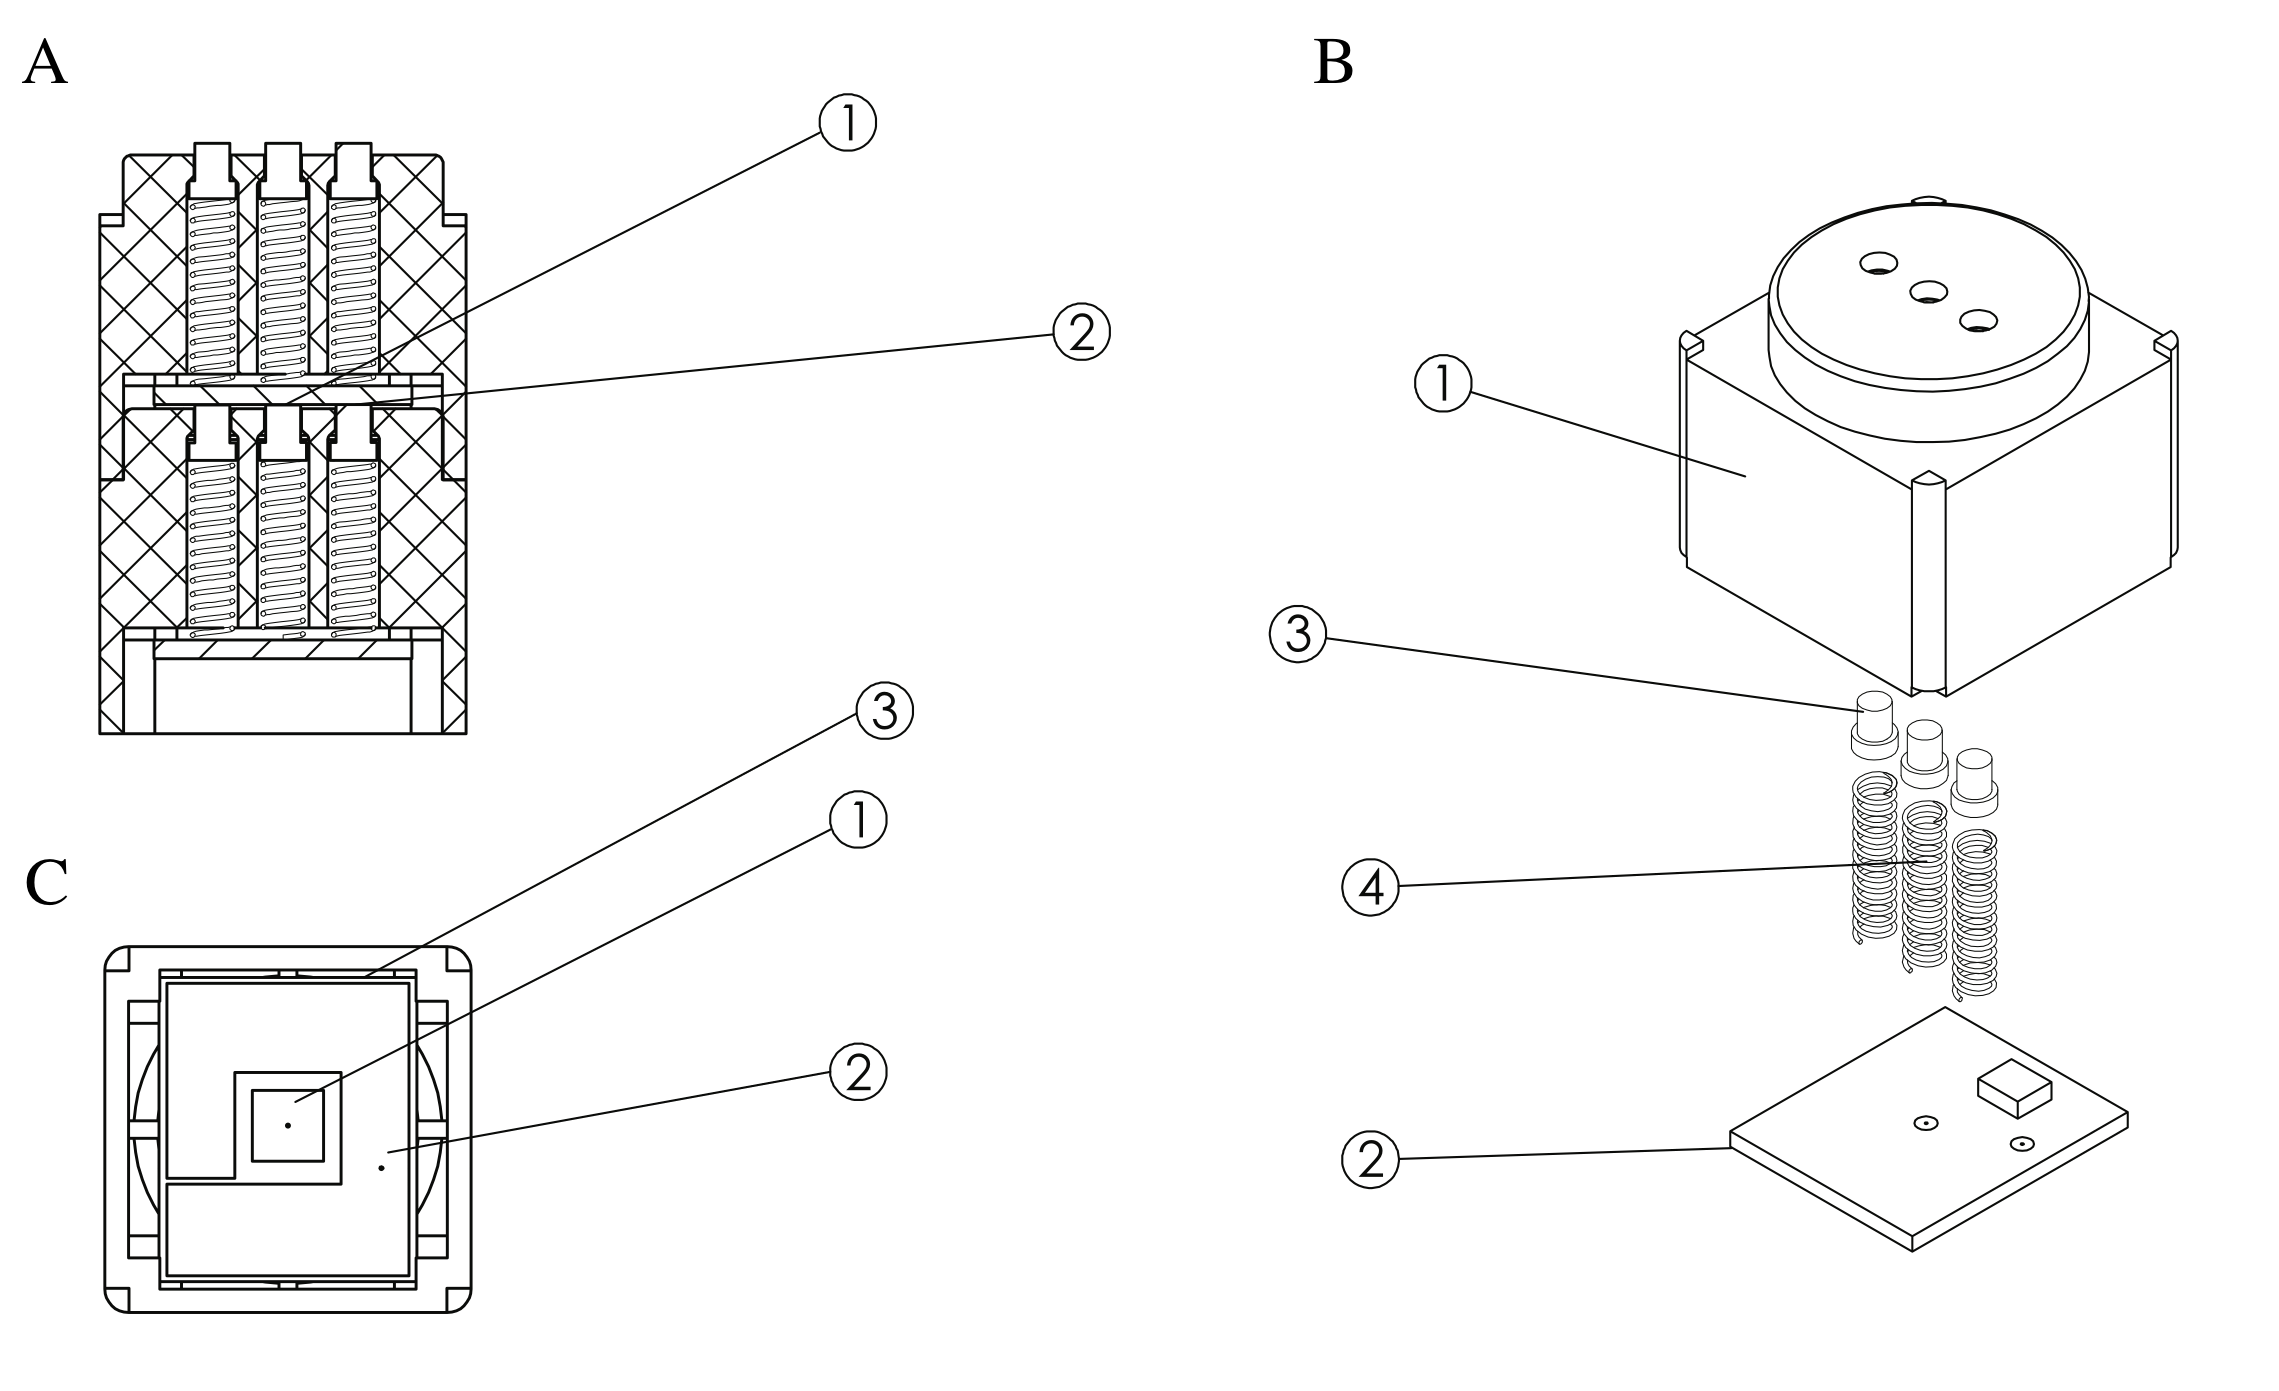
\includegraphics[width=\textwidth]{Figures/single_block}
	\caption{(A) Section view of block connection mechanism (B) Exploded view of block assembly (C) Bottom view of block PCB}
	\label{fig:block}
\end{figure}

Each individual block consists of a plastic shell (Fig. \ref{fig:block} B detail 1) with a square or rectangular block base and one or more cylindrical tops with a series of through holes on its top.  Each through hole contains a protruding electrically conductive contact as shown in Fig. \ref{fig:block} B detail 3. A square, printed circuit board (Fig. \ref{fig:block} B detail 2) is connected via springs (Fig. \ref{fig:block} B detail 4) to the contacts and mounted slightly above the base of the square portion of the block geometry. When a block is placed atop one of the raised cylindrical surfaces or nodes on the grid base, the protruding contacts on the node make a connection with the bottom surface of the lower, square circuit board in the block. This connection provides power to the block’s circuit board as well as enabling communication to other blocks and the base play surface. This communication enables the registration of an individual block’s presence and x-y-z location. 

Subsequent blocks (Fig. \ref{fig:block} A) placed atop a block that is already connected to the grid will receive power through the lower block (which is powered because of its grid connection) and similarly be able to broadcast presence and x-y-z location. The springs mounted between the top and bottom circuit boards provide a robust connection between blocks or between a block and a grid base node as seen in Fig. \ref{fig:block} A Detail 2.  The individually sprung pins  enable the blocks to withstand poor flatness tolerances and height discrepancies inherent to the mating surfaces due to manufacturing processes. Each PCB (Fig. \ref{fig:block} C Detail 3) contains at least two electrically isolated planes where one serves as ground (Fig. \ref{fig:block} C Detail 1) and one provides communication and power (Fig. \ref{fig:block} C Detail 2). In other configurations a third or fourth plane may be necessary in order to provide electrically isolated connections for power, communication, and addressing. 


\subsubsection{Base Subsystem}
The invention also consists of a base grid of rows and columns of nodes of raised cylindrical surfaces onto which individual blocks can be mounted. Each cylindrical surface has 2 to 5 through holes. Each base node has 2 to 5 copper contacts that protrude past the through holes, slightly proud of  the upper surface of the node. The grid base also contains a microcontroller, battery and wireless communication module to broadcast electronic signals to a virtual platform. When any of the individual blocks are placed onto a raised surface on the grid, their presence and row/column or x-y position on the grid is recognized and immediately broadcast to the virtual platform. When stacked atop one another, each block’s position in terms of height (z location) is also broadcast along with its row/column or x-y location.

LEDs have been embedded in the base to provide a variety of different feedback signals to the user.  The primary mode in which the LEDs will operate is to determine the correct orientation of the base.  Additional modes include indicating success or failure within the game, as well as visualizing battery life depletion.

Determining the correct orientation of the base is a key part of the unboxing and setup process, as the base block is preprogrammed to interact with the game software assuming the base to be oriented in a specific way.  An incorrect orientation, as such, would result in a frustrating and confusing gameplay experience.   To facilitate successful orientation, the LEDs, two green and two red, are used to provide visual cues to the user.  The two green LEDs indicate the back side of the base, while the two red LEDs indicate the front.  The colors will correspond to same-color indicators on the screen during game setup.  The user will then rotate the base until the LEDs match what is indicated on the screen.
In addition to aiding in proper setup, the LEDs are used to provide feedback to the user throughout the game.  For example, if the user correctly places the blocks to complete the challenge, the green LEDs flash or illuminate to indicate successful completion of the task.  Conversely, if the user fails to complete the challenge within the constraints set forth, the red LEDs illuminate, indicating a failure to complete the task.  Such phenomena would also occur on the screen, to continue to perpetuate the unity between the physical and virtual games.
The LEDs are also used to inform the user of issues related to the base block itself.  As the batteries begin to get low and need to be charged, the LEDs flash in a specified pattern to indicate to the user that the base should be charged.  Such illumination is also used to indicate when the batteries are too depleted to successfully connect the base to the game, thus alleviating frustration related to troubleshooting why the base is not syncing with the game in a low battery situation.

In another aspect, the invention also consists of a virtual platform that will display a real time virtual image of the block configurations, maintaining persistent communication with the block grid base and updating the virtual image any time a new block configuration is detected.

\subsection{Software}

Block configurations:
1 x 1
2 x 1
3 x 1
2 x 2

Block shapes:
Square Prism
Rectangular Prism
Round Cylinder
Irregular extruded shapes
Other…

Grid variations:
Resolution
Tethered
Wireless (wifi, Bluetooth, RF)

\subsubsection{Interblock Communication Protocol}

\subsubsection{Context Aware Personalization}
Action Primitives for Context Aware Content Personalization
Atoms are novel interface (and abstraction) for expressing physical activities that can be a collection or sequence of “action primitives” to enable content-coupled physical activities. An action primitive encapsulates the actuation, type of input, method of detection, and the interpretation of the input for a particular action. Depending on the perspective of the user and the perspective of the machine, the action primitives have separate meanings.

Action Primitive for Users
User spatial input: where to place a particular block or block type in the block configuration space (the baseboard in this embodiment). Requirement expressed as a guard condition to move to next state in automaton.
User temporal input: when to do a particular step through a sequence of activity (time). Requirement expressed as a guard condition to move to next state in automaton.
User resource constrained input: maximum or minimum  number of allowable inputs. Requirement expressed as a guard condition to move to next state in automaton.
User combinatorial input: heterogeneity requirement in input type, overall metric on action word. Requirement expressed as a guard condition to move to next state in automaton.

Action Primitive for Machine
Action actuation: where to give the user input (position). Can be thought of as an action command in an automaton.
Action detection: what to sense from the user (signal). Can be thought of as a guard condition in an automaton.
Action interpretation: how to interpret what is sensed (encoding). Can be thought of as a labelling function on an accepting state in an automaton.

Composition of action primitives
Event:  Events are triggered by a specific block configuration. Each event can trigger an action and define the set of reachable states. 
Sequence of Events: A particular task may be triggered by a sequence of event rather than a single event. 
Tasks: Tasks are higher level compositions of several events defining a goal.
Experience: Composed of tasks and has a specific objective(s)
Objective: The higher-level goal of a physical activity routine and is the basis for the evaluation of the user






Interaction Modes
Environment Construction and “Toolmaking”
Compositional Constraint
Temporal Constraint
Resource Constraint
Free construction with Digital Persistence
Social mode




\section{CLAIMS}
\begin{itemize}
\item A first toy building block system comprising stacking interlocking rectilinear toy blocks and an autonomous free-standing toy grid base containing an embedded microcontroller and battery that can communicate each block’s position in real time via a wireless data signal such as Bluetooth, WiFi or RF.

\item A first toy building block according to claim 1 wherein the system does not include a camera, vision system, or external means of sensing block orientation and position. 

\item The first toy building block according to claim 1 that is a rectilinear polyhedron toy building block comprising: a top wall; four side walls extending orthogonally away from the top wall to a bottom end of the block, each of the four side walls having an interior surface facing a geometric center of the block and an opposing exterior surface exposed outside of the block.

\item The first toy building block according to claim 1 that can confirm its presence on the toy grid base described in claim 1 through direct electrical contacts that touch one another when a block is stacked on the grid. 

\item The first toy block system according to claim 3 such that the block contains two circuit boards that receive ground, power and signal through two contacts utilizing a Dallas 1-wire chip. Since they utilize power from the grid base, they do not contain a power source on their own, and their construction can be restricted to the simple embedding of circuit boards.

\item The first toy building block according to claim 1 that can confirm its presence atop another block when the bottommost block is placed on the base grid.

\item The first toy building block according to claim 1 that can broadcast wireless signals that map to a virtual representation of the block and grid, updating in real time to show the absence or presence of blocks on the grid.
\end{itemize}

Related Inventions
Is this invention related to a prior invention disclosed to PCI? No
If yes, please provide the docket number and/or title of the related invention(s).
Was the invention developed using any research tools, biological substances, or other proprietary materials obtained from a third party? If so, was there a Material Transfer agreement?

\end{document}
